% THIS IS AN EXAMPLE DOCUMENT FOR VLDB 2012
% based on ACM SIGPROC-SP.TEX VERSION 2.7
% Modified by  Gerald Weber <gerald@cs.auckland.ac.nz>
% Removed the requirement to include *bbl file in here. (AhmetSacan, Sep2012)
% Fixed the equation on page 3 to prevent line overflow. (AhmetSacan, Sep2012)

\documentclass{vldb}
\usepackage{graphicx}
\usepackage{balance}  % for  \balance command ON LAST PAGE  (only there!)
\usepackage{color}
\usepackage{cleveref}

\begin{document}

% ****************** TITLE ****************************************

\title{Two Phase Commit on Persistent Key Value Store with Data Replication}

% possible, but not really needed or used for PVLDB:
\subtitle{6.824 Distributed Systems Final Project}
%\titlenote{A full version of this paper is available as\textit{Author's Guide to Preparing ACM SIG Proceedings Using \LaTeX$2_\epsilon$\ and BibTeX} at \texttt{www.acm.org/eaddress.htm}}}

% ****************** AUTHORS **************************************

% You need the command \numberofauthors to handle the 'placement
% and alignment' of the authors beneath the title.
%
% For aesthetic reasons, we recommend 'three authors at a time'
% i.e. three 'name/affiliation blocks' be placed beneath the title.
%
% NOTE: You are NOT restricted in how many 'rows' of
% "name/affiliations" may appear. We just ask that you restrict
% the number of 'columns' to three.
%
% Because of the available 'opening page real-estate'
% we ask you to refrain from putting more than six authors
% (two rows with three columns) beneath the article title.
% More than six makes the first-page appear very cluttered indeed.
%
% Use the \alignauthor commands to handle the names
% and affiliations for an 'aesthetic maximum' of six authors.
% Add names, affiliations, addresses for
% the seventh etc. author(s) as the argument for the
% \additionalauthors command.
% These 'additional authors' will be output/set for you
% without further effort on your part as the last section in
% the body of your article BEFORE References or any Appendices.

\numberofauthors{2} %  in this sample file, there are a *total*
% of EIGHT authors. SIX appear on the 'first-page' (for formatting
% reasons) and the remaining two appear in the \additionalauthors section.

\author{
% You can go ahead and credit any number of authors here,
% e.g. one 'row of three' or two rows (consisting of one row of three
% and a second row of one, two or three).
%
% The command \alignauthor (no curly braces needed) should
% precede each author name, affiliation/snail-mail address and
% e-mail address. Additionally, tag each line of
% affiliation/address with \affaddr, and tag the
% e-mail address with \email.
%
% 1st. author
\alignauthor
Xiangyao Yu\\
       \affaddr{Massachusetts Institute of Technology}\\
       \affaddr{32 Vassar Avenue}\\
       \affaddr{Cambridge, MA}\\
       \email{yxy@mit.edu}
% 2nd. author
\alignauthor
Shuotao Xu\\
       \affaddr{Massachusetts Institute of Technology}\\
       \affaddr{32 Vassar Avenue}\\
       \affaddr{Cambridge, MA}\\
       \email{shuotao@mit.edu}
}


\maketitle

\begin{abstract}
  We implemented a distributed transaction processing system where data is
  partitioned and mapped to different shards. All shards are replicated to enhance
  the availability and durability of the system.  The database model is simple
  key-value store inherited from Lab 4.  The objectives of the project are 1) to
  process transaction using two phase commit and guarantee atomic execution, 2) to
  persistently store data and server status on disk to tolerate server failures. The
  requests of a transaction consist of GET, PUT, and ADD. To simplify implementation,
  the only scenario of aborting a transaction is that it has an add request that
  results a negative value. Firstly, we implemented a coarse-grained locking scheme
  where a transaction locks the groups it touches. In order to achieve better
  performance gains, we later refined our system with a fine-grained locking scheme
  where a transaction locks the keys it touches. Secondly, we implemented test cases
  to verify the correctness of the system under different failure scenarios including
  unreliable networks and server failures. Lastly we benchmark our system with
  synthetic workloads that varies with parameters like distribution of number of
  groups a transaction accesses, read/write ratios of a transaction, number of
  clients and so on.
\end{abstract}


%\section{Introduction}

%foo


\section{Implementation Details}

Our persistent key value store is constructed such that each key of 
type string is mapped to a value of type integer. We confined the type 
of values to integer to allow arithmetic operations on the key-value 
pairs. The data of our systems are partitioned into different shards.  
A group of servers are responsible for a distinct subset of shards, 
and all the data within a group are replicated. Our system supports 
atomic transactions, where a transaction is an ordered group of 
requests such as puts, gets and etc. We also support persistency, 
where all committed transactions are recorded to disk. Our persistent 
key-value store can model applications like an inventory management 
system or a bank account system.

\subsection{Transaction Support}
\label{sec:txn}

Our system supports transaction consisting of requests of PUTs, GETs, 
and ADDs.
\begin{itemize} \item a PUT updates the value associated with the key
\item a GET returns the value associated with the key
\item an ADD adds a value (could be negative) to the previous value 
associated with the key
\end{itemize}

In particularly, the transaction support of our system ensures the 
following properties. 

\textbf{Consistency} Our system allows multiple clients to send 
transactions concurrently. Specifically, our database enforce 
sequential consistency such that the effects of concurrent 
transactions appears as some sequential order.  To enable sequential 
consistency, the client should lock the groups that a transaction 
touches before execution. And since we will have multiple servers 
within each group, we will ensure consistency inside the group with 
Paxos, to guarantee a global ordering of the operations within a 
group.

\textbf{Atomicity} The transactions need also be atomic, i.e. either 
all of the requests of the transaction are executed or none are 
executed. We ensure atomicity of the transaction with two phase commit 
protocol.

\textbf{Persistency} All the effects of a committed transaction on key 
value store are written on disk.

\textbf{Fault-tolerant} Our system ensures the transaction processing 
is fault-tolerant. On the server sides, the Paxos implementation in 
Lab 3 has already ensured tolerance under network failures. In our 
project, we will modified Lab 3 such that Paxos can also handle server 
crashes. On client side, we will also record its transaction 
processing status on disk, so that after crash, the client will know 
at which point it was processing the transaction.

\subsubsection{Persistent Paxos}

We made the Paxos persistent so that it can tolerate server crash.

Whenever any of the propose number(n\_p), accepted number(n\_a) and 
accepted value(v\_a) is modified, all of them are written to the file 
system with the file name in the following format: 
\textit{SERVERNAME\_INS\#.txt}.

When the Paxos log is truncated, the corresponding files are also 
deleted. When a server reboots after failure, it will reconstruct the 
Paxos instances by reading from the file system. We use a lazy 
reconstruction approach where an instance is read and reconstructed 
only when it is touched.

Moreover, we added a new function call, Poll(seq int), to the Paxos, 
to peek the status of a Paxo instance at some sequence number. When 
Poll(seq int) is called, the Paxos server first checks locally if the 
Paxos instance of sequence number \textit{seq} has been decided (by 
calling Status()). If not, RPCs are sent to peer servers and the 
status of the instance is returned. Note that Poll() is different
from Status() since Status() only checks the Paxos instance on local 
server.

Poll is used to check whether a particular instance has been decided.  
This simplifies our system implementation as explained in 
Section~\ref{sec:lock}.


\subsubsection{Locking Scheme}
\label{sec:lock}

We uses locking to ensure sequential consistency of concurrent 
transactions.

Transactions are initiated at the client side. A client breaks down a 
transaction, and sends the requests to a server in the corresponding 
group. Upon receiving the requests, the server will start a Paxos 
instance to agree on the transaction. This Paxos instance also does 
the proper locking for the transaction to guarantee mutual exclusive.

To avoid deadlocks, the clients should send requests to the groups 
sequentially following a fixed order, such as the order of increasing 
group IDs. Groups with larger gids are locked only after groups with 
smaller gids are locked. This prevents the scenario where two 
transactions each locks a group and requests to lock the other's 
group.

In our implementation, locking can happen in two differnt 
granularities, \textit{per-group locking} and \textit{per-row 
locking}. 

In \textit{per-group locking}, a transaction locks a whole group if 
any data in that group is touched (read or write). Another transaction 
can only access the same group until the first has released the lock.  
The advantage of this implementation is its simplicity. But the 
performance is sacrificed since only one transaction can access a 
group at any time. 

In \textit{per-row locking}, a transaction only locks the rows it 
needs to access. Two types of locking are supported: shared lock for 
GET requests and exclusive lock for PUT or ADD requests. Multiple GET 
requests from different transactions can share lock the same record at 
the same time. When a transaction reaches a group, it will first try 
to lock the records it will access within the group. If any lock 
fails, no lock should happen and a lock failure message is replied to 
the client. Compared to per-group locking, this approach exploits much 
more concurrency and should provide higher performance 
(\cref{sec:eval})

To tolerate failures, we have Paxos handle failures on server side. On 
client side, when a transaction starts, the client will record its 
status as \textit{started} on disk. When all groups are properly 
locked, the on-disk status of the client changes to \textit{locked}.

The servers will periodically use Poll() to catch up in the Paxos log 
with other replicas. Otherwise, there is possibility that some of the 
servers will be left far behind in the Paxos log and take a long time 
to catch up. For example, after a client locks a server for a 
transaction, it seeks other servers to execute two phase commit in
Section~\ref{sec:2pc}. Later the client send request to this server to 
lock for a new transaction. That server still grabs lock from previous 
transaction, rejects the new transaction request and waits for the 
prepare message of previous transaction, which will never come. In 
this case, the server stalls, and the new transaction can not
proceed.

This is the first step of transaction processing from client's 
perspective, we call it \textit{insert transaction}.

\subsubsection{Two Phase Commit}
\label{sec:2pc}

After client hears from all groups that the servers have been properly 
locked for the transaction, it initializes two-phase commit(2pc) 
protocol\cite{mohan86} as described in \cref{fig:2pc}, where the records with 
* are written into non-volatile storage.

\begin{figure}[h!]
  \centering
  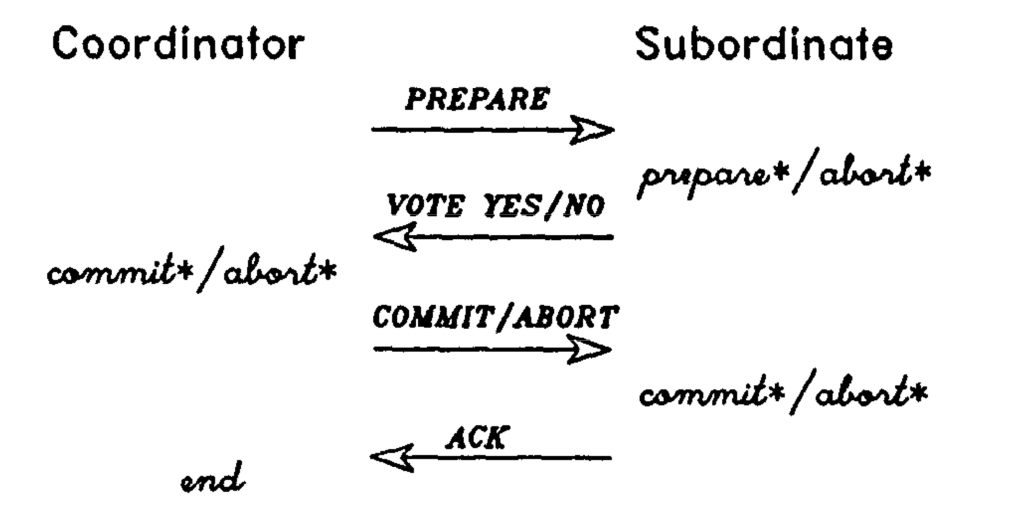
\includegraphics[width = 0.8\linewidth]{figs/2PC.pdf}
  \caption{Two Phase Commit Protocol}
  \label{fig:2pc}
\end{figure}

The client will first send prepare messages to all the groups that a 
transaction involves in parallel to make sure the transaction can be 
executed. The servers pre-run the transaction. And if there is an ADD 
request that results negative integer, it responses abort. Otherwise, 
the server responses prepare\_ok. The client waits for all prepare 
responses from different groups. And depends on the prepare messages, 
client 1) sends out reply to application and 2) either sends out
commit or abort message to servers. After servers sees commit, it will 
write the result of the transaction into persistent storage.

As shown in Figure \cref{fig:2pc}, two-phase commit requires the 
coordinator(client) to write once to the persistent storage
(commit/abort) and subordinate(servers) to write twice to the 
persistent storage (prepare\_ok/abort and commit/abort). In our
implementation, the server always need to make consensus on those two 
messages through Paxos. Since our Paxos is already persistent, two 
phase commit is automatically achieved at the server side. 

At the client side, we added an extra disk operation to make the state 
of the current transaction persistent. When a client reboots, it will 
first read the disk for the latest state before it crashed and repeat 
the last operation if necessary. 

The servers, on the other hand, should passively wait for the client’s 
requests to insert Paxos instance. So it does not have to recover the 
states up to date immediately. We take a lazy approach to recover the 
servers: only replay Paxos log and recover the states when the 
incoming request depends on it. For example, a server after reboot may 
receive a commit request without knowing the result of the 
transaction. It will replay the Paxos log at this point and read the 
transaction results from the log and serve the commit request.

The prepare and commit phases in 2pc are the second and third steps of 
transaction processing from client's perspective.

\subsection{Testing}

We implemented various test cases to make sure our implementation 
works correctly. In general, our tests fall into two categories: 
\textit{transaction testing} and \textit{2pc testing}. 

\subsubsection{Transaction Support}

This test is to make sure that our database satisfies atomicity and 
consistency, i.e., the requirement of the notion of transaction. For 
atomicity, we need to make sure that a transaction either completely 
commits or completely aborts. Partial transactions are not allowed.  
For consistency, the database should support multiple clients sending 
requests concurrently and the results are equivalent to some order of 
sequential execution. We designed the following test cases 
accordingly.

\textbf{Test 1} A single client sends requests to three groups of servers where each
group contains 3 servers. One of the requests will add a negative value to the
database to make record less than 0 and thus should abort. The test verifies that all
the changes of the aborted transaction are rolled back. Both reliable and unreliable
networks are tested.

\textbf{Test 2} Initially, each group has a record with value 10.  Three clients send
requests to all the 3 groups to add -1 to the corresponding record. Within a certain
transaction, the values returned from all the groups should be the same. And values
returned by different transactions should be different. Both reliable and unreliable
networks are tested.

\subsubsection{Two Phase Commit}

To test that our \textit{two-phase commit} protocol is correct we need to manually
crash the system at different point and reboot the system to see if it can still run
properly. A \textit{failpoint} parameter is passed into both the client and the
server when the transactions run.  When the machine(client/server) runs into the
position indicated by the \textit{failpoint}, the machine should delete all the
information stored in the main memory. The data stored on the disk, however, is
preserved.

After faiure, the Reboot() function in either the client or the server 
is called to recover the process. And if the system is correctly 
implemented, all the transactions should behave properly.

The following failure points are considered in the test and they are 
tested individually.

\textbf{Client Side}

Case 1: Client fails after locking all the groups but before sending 
out prepare requests.

\textbf{Server Side}

Case 1: Server fails before writing the prepare record to disk.

Case 2: Server fails after writing the prepare record to disk but 
before replying the to the client.

Case 3: Server fails after replying the prepare state to the client.

Case 4: Server fails after writing the commit record to disk but 
before replying to the client.

Fianlly, we also tested the persistent database storage. In this test, 
the system is first loaded with data and then the whole system 
crashes. After reboot, the system should recover all the missing data 
by reading from the disks. 

\section{Performance Results}
\label{sec:eval}

In this section, our system is evaluated in several different aspects.  
In particular, we will first evaluate the overhead of using paxos to 
reach consensus within a group. Then we evaluate the overhead of disk 
operations in our 2PC. Finally, we compare the two concurrency control 
schemes introduced in \cref{sec:txn}. All the experiments are carried 

\subsection{Overhead of Paxos}

To evaluate the overhead of paxos protocol between replicas, we assume 
a single client and a single group.  In the first case, the group 
contains only a single server which processes the request alone.  In 
the second case, the group contains three servers and each request 
should go through the paxos protocol.  The difference between the 
performance (\cref{fig:paxos-persistent}) shows the overhead of paxos 
protocol. 

\begin{figure}[t!]
	\centering
	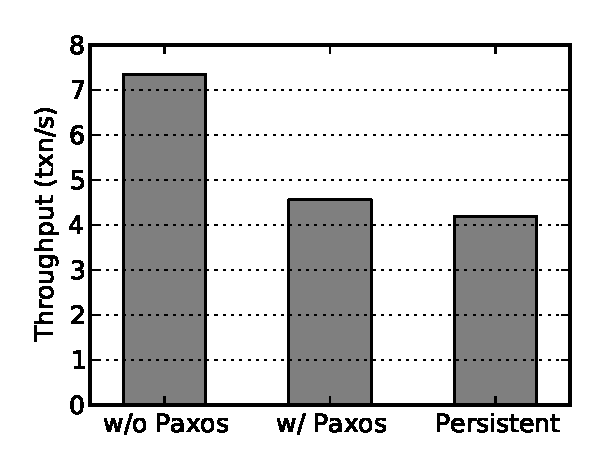
\includegraphics[width=0.6\columnwidth]{figs/paxos_persistent.pdf}
	\caption{
		Performance overhead of paxos protocol and persistent storage.
	}
	\label{fig:paxos-persistent}
\end{figure}

\cref{fig:paxos-persistent} also shows the overhead of writing the 
records to persistent storage in order to tolerate system crashes. It 
turns out that the disk writing overhead is smaller than the overhead 
of paxos protocol. 

\subsection{Locking Granularity}

\begin{figure}[t!]
	\centering
	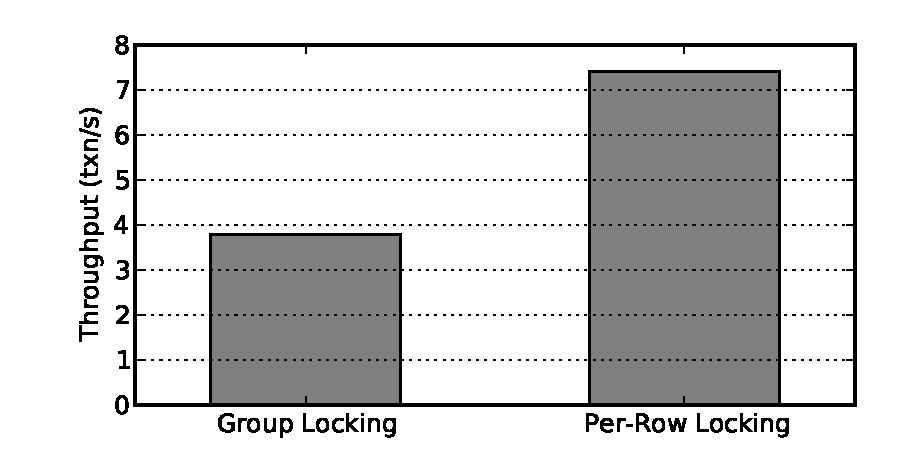
\includegraphics[width=0.6\columnwidth]{figs/locking_granularity.pdf}
	\caption{
		Performance comparison between different locking granularity.
	}
	\label{fig:locking-granularity}
\end{figure}

\cref{fig:locking-granularity} shows the performance comparison 
between per-group locking vs. per-row locking. The experiment involves 
three clients and three groups with three servers in each group. The 
database contains 1000 records. Each transaction uniform randomly 
touches six records, two in each group. 

Clearly, per-row locking significantly outperforms per-group locking.  
Per-row locking allows two transactions to run concurrently as long as 
their data sets do not overlap. In our setting, most transactions 
access disjoint sets of data which is the best scenario for per-row 
locking. 

\section{Discussion}

To summarize, our project is built on top of Lab4. We enhanced the 
pure key-value storage engine to a transactional processing engine.
Then, persistent paxos and persistent data storage are added. And 
two-phase commit is supported on top of these. 

We also implemented various test cases to verify the correctness of 
our implementation. Finally, we evaluated the performance of our 
system and studied tradeoffs in different design decisions.

From the project, we learned that Paxos is a very expensive protocol that it
supersedes all overheads of 2pc and disk operations. In the future, optimization could
be done on Paxos, to further increase our system's performance.

%\textcolor{red}{TODO : add some thoughts? like what we learned?}

\bibliographystyle{abbrv}
\bibliography{report}  % vldb_sample.bib is the name of the 
% Bibliography in this case
% You must have a proper ".bib" file
%  and remember to run:
% latex bibtex latex latex
% to resolve all references

%\subsection{References}



\end{document}
